\section{Modelisation}
    \subsection{Formalisme}
    The objective of our work is to automate a car so that it is able to go from point A to point B while avoiding obstacles.
    The kinematics of the car is modelled by the following equations:
        \begin{equation}
            \label{eqn:constrains}
            \begin{cases}
                (\mathit{i}) & \dot{x} = v\cos{\phi} \\
                (\mathit{ii}) & \dot{x} = v\sin{\phi} \\
                (\mathit{iii}) & \phi=u_{\pi_{\theta}} \\
                (\mathit{iv}) &  v = k \\
               
            \end{cases}
        \end{equation}
    At first, I tried to control only the steering angle of the car. Thus $u_{\pi_{\theta}}$ represents the $\phi$ output taken via a policy $\pi_{\theta}$.
    The robot is also equipped with three sonars, one frontal and two lateral, which allow to visualize its environment.

    \subsection{Simulation}
    Once the kinematics were defined, I had to simulate the robot and obtain a visual rendering. I used the Kivy library of python. 
    Kivy is a free and open source Python framework for developing mobile apps and other multitouch application software with a natural user interface.
    The objective was to have a visual rendering of the robot's evolution, but also to be able to interact with the environment via a man-machine interface. 
    Once the simulation is launched, a window opens and the robot evolves in its environment. The operator can interact with the robot's environment by creating walls that he can draw with the mouse. 
    There is also a button to erase all the walls on the map to rebuild others and see if the robot is able to generalise its behaviour in any type of environment.
    \begin{figure}[!htb]
        \centering
        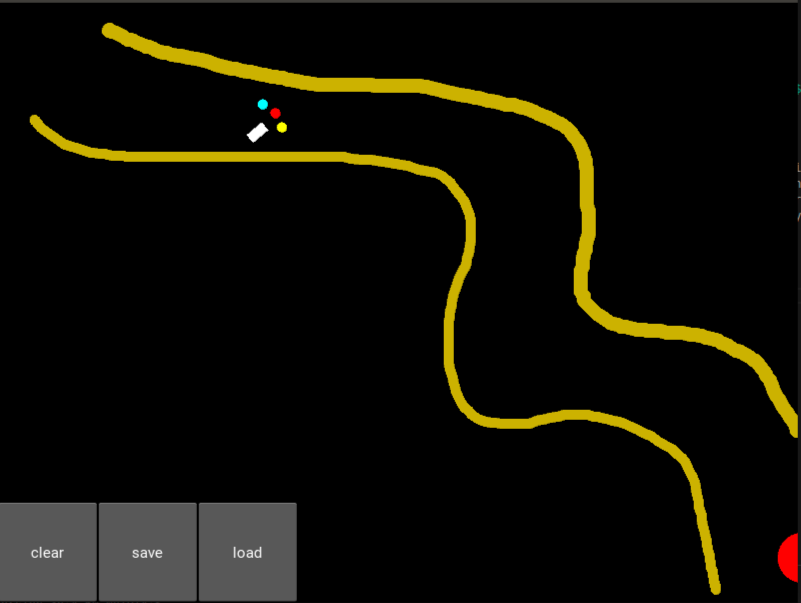
\includegraphics[width=0.4\textwidth]{imgs/simulator.png}
        \caption{\label{fig:simulation} Simulation of the system}
    \end{figure}


    As can be seen in the figure. The car is represented by a white square. The sonars of the car are represented by the three circles at the front of the car.
    
    \begin{figure}[!htb]
        \centering
        
\includegraphics[width=0.2\textwidth]{imgs/robot.png}
        \caption{\label{fig:simulation} Robot sonars}
    \end{figure}
    

    The walls are represented by the yellow lines. And the objective of the robot is represented by the red dot. 
    At first, the robot can cross walls but when it does so its speed decreases and it gets a negative reward because it has crossed the wall and because it will arrive less quickly at its target.
